\documentclass[tikz,border=7pt]{standalone}

\usepackage{amsmath}
\usepackage{bm}
\usetikzlibrary{arrows.meta,calc}

% Colours match the Acrobot and general multibody figures.
\definecolor{frameblue}{RGB}{48,52,255}
\definecolor{rhovector}{RGB}{238,132,24}
\definecolor{linkfill}{RGB}{249,249,249}
\definecolor{linkshade}{RGB}{222,226,231}

\tikzset{
  cylinderbody/.style={
    draw=black,
    line width=0.85pt
  },
  frameaxis/.style={
    draw=frameblue,
    line width=1.15pt,
    line cap=round,
    -{Stealth[length=2.35mm,width=1.85mm]}
  },
  rhoarrow/.style={
    draw=rhovector,
    line width=1.20pt,
    line cap=round,
    -{Stealth[length=2.35mm,width=1.85mm]}
  }
}

\begin{document}
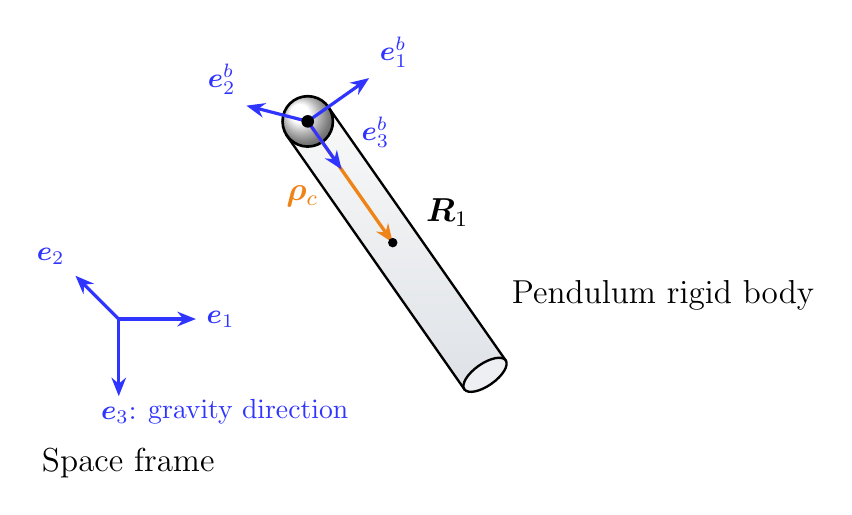
\begin{tikzpicture}[x=1cm,y=1cm]

  % The body attitude shown here is a rotation about the inertial e_2-axis.
  % Consequently, the body b_3-axis and the cylinder axis point downwards
  % and to the right. Both the space and body frames have their physical
  % origin at the fixed pivot; the space frame is repeated below for clarity.
  \coordinate (B) at (0.15,1.55);
  \coordinate (P) at (0.25,1.41);
  \coordinate (C) at (1.33,-0.13);
  \coordinate (E) at (2.51,-1.81);
  \coordinate (G) at (-2.15,-1.10);

  % Cylindrical rigid body: l=1 m, r=0.05 m in the numerical evaluation.
  % It is drawn first so that the geometric vectors and frames remain visible.
  \begin{scope}[shift={(B)},rotate=-55]
    \shade[
      cylinderbody,
      top color=linkfill,
      bottom color=linkshade
    ] (0.16,-0.32) rectangle (4.10,0.32);
    \path[
      cylinderbody,
      fill=linkshade!55
    ] (4.10,0) ellipse[x radius=0.14,y radius=0.32];
    \draw[black!65,line width=0.55pt]
      (0.16,0) ellipse[x radius=0.14,y radius=0.32];
  \end{scope}

  % Fixed frictionless spherical pivot, drawn before the body frame so the axes remain visible.
  \shade[
    ball color=white,
    draw=black,
    line width=0.95pt
  ] (P) circle[radius=0.32];

  % Body-fixed center-of-mass vector. Since rho_c=(l/2)e_3^b, it is
  % collinear with the cylinder and the body b_3-axis.
  \draw[rhoarrow] (P) -- (C);
  \fill[black] (C) circle[radius=0.060];
  \node[text=rhovector,font=\large,anchor=south east]
    at ($(P)!0.59!(C)+(-0.38,-0.30)$) {$\bm{\rho}_{c}$};

  % Body-fixed, right-handed three-dimensional frame at the pivot.
  % The projected axes correspond to a rotation about e_2:
  % b_1 points up-right, b_2 up-left, and b_3 along the cylinder.
  \draw[frameaxis] (P) -- ++(0.78,0.55)
    node[text=frameblue,font=\normalsize,anchor=south west] {$\bm{e}^b_1$};
  \draw[frameaxis] (P) -- ++(-0.78,0.20)
    node[text=frameblue,font=\normalsize,anchor=south east] {$\bm{e}^b_2$};
  \draw[frameaxis] (P) -- ++(0.43,-0.61);
  \node[text=frameblue,font=\normalsize,anchor=west]
    at ($(P)+(0.56,-0.14)$) {$\bm{e}^b_3$};

  % Pivot center point, drawn last so it remains above the body frame.
  \fill[black] (P) circle[radius=0.080];

  % The rotation matrix is the only configuration variable.
  \node[font=\large,anchor=west] at (1.63,0.25) {$\bm{R}_{1}$};
  \node[font=\large,anchor=west] at (2.72,-0.80) {Pendulum rigid body};

  % Space-fixed, right-handed three-dimensional reference frame.
  % The thesis defines e_3=[0,0,1]^T as the gravity direction; hence it
  % points vertically downwards in this drawing.
  \draw[frameaxis] (G) -- ++(0.98,0)
    node[text=frameblue,font=\normalsize,anchor=west] {$\bm{e}_1$};
  \draw[frameaxis] (G) -- ++(-0.55,0.55)
    node[text=frameblue,font=\normalsize,anchor=south east] {$\bm{e}_2$};
  \draw[frameaxis] (G) -- ++(0,-0.98)
    node[text=frameblue,font=\normalsize,anchor=north] {$\bm{e}_3$:};
  \node[font=\large,anchor=north] at ($(G)+(0.12,-1.52)$) {Space frame};
  \node[text=frameblue,font=\normalsize,anchor=west]
    at ($(G)+(0.25,-1.18)$) {gravity direction};

\end{tikzpicture}
\end{document}
